\documentclass[12pt]{article}
\usepackage[T1]{fontenc}
\usepackage[utf8x]{inputenc}
\usepackage[usenames,dvipsnames]{xcolor}
\usepackage{multirow}
\usepackage{minted}
\usepackage{fancyhdr}
\usepackage{setspace}
\usepackage{caption, newfloat}
\usepackage{upquote}
\usepackage[color, matrix, arrow]{xy}
\usepackage{mathtools}
\usepackage{graphicx}

\renewcommand{\contentsname}{Topics}
\renewcommand*{\addcontentsline}[3]{\addtocontents{#1}{\protect\contentsline{#2}{#3}{}}}

\setlength{\marginparwidth}{1.2in}
\let\oldmarginpar\marginpar
\renewcommand\marginpar[1]{\-\oldmarginpar[\raggedleft\footnotesize #1]%
{\raggedright\footnotesize #1}}

\newcommand{\todo}[1]{\marginpar{\color{red} #1}}

\newcommand{\adj}[1]{{\color{blue} #1}}

\newcommand{\say}[1]{{\color{magenta} #1}}

\newenvironment{code}[3][false]
 {
  \VerbatimEnvironment

  \begin{lstlisting}
  \caption{#3}
  \begin{minted}[linenos=#1]{#2}}
 {
  \end{minted}
  \end{lstlisting}
 }


\DeclareFloatingEnvironment[placement={H}]{lstlisting}[Example][List of Listings]
\captionsetup[lstlisting]{box=colorbox,boxcolor=RoyalBlue,font={color=white, bf},labelsep=endash,skip=5pt}

\setlength{\headheight}{15pt}

\begin{document}

\title{Lecture 2: JavaScript and the HTML DOM}
\author{Nick Hynes}
\date{January 14, 2014}

\maketitle

\begin{spacing}{0}
\setcounter{tocdepth}{1}
\tableofcontents
\end{spacing}

\section{HTML}
\textless rhetorical-question\textgreater So, what is HTML?\textless /rhetorical-question\textgreater{} HTML is a \textbf{M}arkup \textbf{L}anguage designed for use with \textbf{H}yper\textbf{T}ext, or text that contains links to other (hyper)text. Practically, HTML is a language used to create web pages. This also means that HTML something of a GUI language for JavaScript!
\par
Markup languages are designed to allow syntactic description of data to change its display or semantics (or both). As a markup language, HTML is very similar to other such languages with which you may be familiar; XML (eXtensible Markup Language), Markdown, and LaTeX are notable examples. It is important to note that, unlike LaTeX and Markdown, HTML, especially HTML5, the latest version, focuses more on the \emph{semantics} of a document than its presentation.
\par
Great! Now that you know what HTML does and why it's used, let's look at how you actually use it!
\subsection{Syntax}
An HTML page is constructed by nesting HTML tags or text inside of other HTML tags. A general HTML tag takes the following format:
\begin{Verbatim}[frame=single]
<tagname attribute="value" data-customattribute="value">
  More HTML tags or text
</tagname>
\end{Verbatim}
Although the attributes are optional, the start and end tags are required. Here's an example of a page div[ision] containing a paragraph on HTML escape characters:
\begin{Verbatim}
<div>
  <p>
    You can make the literal greater than and less than symbols
    using &amp;gt; and &amp;lt;, respectively. The ampersand is
    the escape character, so printing a literal ampersand
    (as we are doing here) requires &amp;. Remember to include
    the semicolon!
  </p> 
</div>
\end{Verbatim}
Tags that may not contain HTML, namely \texttt{meta}, \texttt{img}, \texttt{br}, and \texttt{hr}, are specified using just the start tag.
\begin{Verbatim}[frame=single]
<tagname attribute="value" data-customattribute="value">
\end{Verbatim}
For instance,
\begin{Verbatim}
<img src="http://web.mit.edu/img/MIT_logo.gif" alt="MIT logo">
\end{Verbatim}
creates an image element with the MIT logo as the source and ``MIT logo'' as the alt (mouseover/screen reader) text.
\par
With tags in mind, let's look at a basic HTML page and go two for two on ``hello world'' examples:
\begin{code}[true]{html}{HTML says ``Hello!''}
<!DOCTYPE html> <!-- specifies HTML5 standards mode -->
<html>
  <head>
    <!-- Page metadata (e.g. title, styles) lives here -->
  </head>
  <body>
    <!-- Display elements and document content goes here -->
    <h1>Hello, world!</h1> <!-- A top-level heading -->
  </body>
</html>
\end{code}
The most important part of this example, by far, is the first line: the \emph{doctype}. This signals to the browser that the document contains HTML5 and should be rendered according to the HTML5 specification. The page will, thus, be rendered in the same way by all compliant browsers (in a perfect world). If this is omitted, the document will be rendered in ``quirks mode,'' in which the browser tries its best to display what it thinks the author meant, which may or may not be correct. The next most important part is on line 2 and 9: this is the that that defines the HTML root element. Everything inside \texttt{<html>} and \texttt{</html>} will be treated as---you guessed it---HTML. The two elements that \texttt{html} may contain are \texttt{head} and \texttt{body}. The former contains information about the page itself and its display properties (styling) and the latter contains the actual elements to display.
\par
At this point, you may be thinking: ``Okay, that's nice, but how am I supposed to run my scripts?'' If this is, in fact, the case, then you raise a very important question. However, you may put yourself at ease since you will now be introduced to the almighty \texttt{<script>} tag!


\subsection{The \texttt{<script>} tag}
The \texttt{<script>} tag allows scripts (JavaScripts, to be exact) to be embedded directly into the page or loaded from an external file. The \texttt{<script>} tag is similar to other content-containing tags in that it must possess both a start and end tag. However, in the case of inline (i.e. non-external) scripts, the inner HTML of the tag is parsed and executed as JavaScript. Here's an example:

\begin{lstlisting}
\caption{Scriptacular scripts!}
\begin{minted}{html}
<script type='application/javascript'>
  console.log('I am a script running directly in the page.');
</script>

<script type='application/javascript' src='external_script.js'>
//Anything here is ignored
</script>
\end{minted}
\vspace{0ex}
\begin{minted}{javascript}
/* external_script.js */
//Note that this file does not contain <script> tags
console.log("I am a script loaded from an external file!");
\end{minted}
\end{lstlisting}
Let's look at these two tags more closely. Notice how each has its \texttt{type} attribute set to \texttt{text/javascript}. This signals to the browser that the script is JavaScript and should be run as such. Additionally, the \texttt{src}, or source, attribute of the second tag specifies the location of the JavaScript file. While, in this case, \texttt{src} is pointing to a file named ``external\_script.js'' located in the same directory (folder) as the loading page, \texttt{src} may be an absolute location specified by a URL using \texttt{http://} or a relative path using any number of \texttt{../}, meaning ``go up one directory.''
\begin{code}{html}{Relative paths are absolutely amazing!}
<!-- 
HTML loaded from http://introjsiap.com/examples/js/index.html
-->

<script type='application/javascript' src='../../myfile.js'>
//Points to http://introjsiap.com/myfile.js
</script>

<script type='application/javascript'
src='http://introjsiap.com/scripts/myfile.js'>
//Points to http://introjsiap.com/scripts/myfile.js
</script>
\end{code}
As far as the placement of the \texttt{<script>} tags in the HTML document is concerned, they are valid anywhere in the \texttt{<head>} and \texttt{<body>} tags. However, there are a few choice locations to use that minimize page load times. In particular, \texttt{<script>}s should go towards the bottom of the the \texttt{<head>} tag if the script is involved in the rendering of the page or towards the bottom of the \texttt{body} tag, otherwise. This is due to HTML pages being loaded from the ``top-down'' and scripts blocking the loading of other resources.
\begin{code}{html}{We want to know: where does the \texttt{<script>} go?}
<!DOCTYPE html>
<html>
  <head>
    <!-- styles, metadata, title, etc. -->
    <!-- scripts that draw/render/create the page go here -->
    <script type='application/javascript'></script>
  </head>
  <body>
    <p>Other HTML elements and text</p>
    <!-- other scripts go here -->
    <script type='application/javascript'></script>
  </body>
</html>
\end{code}

\subsection{The HTML DOM}
The HTML Document Object Model is an abstract, tree-like representation of the marked-up text. The nesting of HTML elements produces a hierarchy that describes the structure of the document. Intuitively, the relationships between elements, also called nodes, are described using the terms \emph{parent}, \emph{child}, and \emph{sibling}.
\par
In the following example, we will create an HTML document titled ``HTML!'' that contains a bulleted list containing three items and examine the resulting DOM.
\begin{code}{html}{In the domain of the DOM}
<html>
  <head>
    <title>HTML!</title>
    <script type='application/javascript' src='draw_page.js'>
    </script>
  </head>
  <body>
    <ul> <!-- an unordered list -->
      <li>List item 1</li>
      <li>List item 2</li>
      <li>List item 3</li>
    </ul>
  </body>
</html>
\end{code}
\begin{displaymath}
    \xymatrix{
      & & \texttt{<html>} \ar@{-}[dl] \ar@{-}[dr] & \\
      & \texttt{<head>} \ar@{-}[dl] \ar@{-}[d] & & \texttt{<body>} \ar@{-}[d] \\
      \texttt{<title>} \ar@{-}[d] & \texttt{<script>} & & \texttt{<ul>} \ar@{-}[dl] \ar@{-}[d] \ar@{-}[dr] \\
      \text{HTML!} & & \texttt{<li>} \ar@{-}[d] & \texttt{<li>} \ar@{-}[d] & \texttt{<li>} \ar@{-}[d] \\
      & & \text{List item 1} & \text{List item 2} & \text{List item 3} \\
    }
\end{displaymath}
\\
\par
This is about as complicated as the structure of an HTML document is going to get. Of course, the trick is in knowing where to put the elements in order to make the page display properly. There are two important things to observe about this structure, however. The first is that a node contains references to its parent node and all of its children, but  not its siblings. The other is that the text ``leaves'' of the DOM tree---``HTML'', and ``List item $n$'' in the example---are known as \emph{text nodes}, but it's rare that they're ever created or referred to as such since it is more convenient to treat them as their parent's \emph{inner HTMl}.

\subsection*{A template, for your convenience}
\begin{code}{html}{The HTML page to begin all HTML pages}
<!DOCTYPE html>
<html>
  <head>
    <title>The title of the page</title>
    <meta charset='utf-8'> <!-- the text encoding -->
  </head>
  <body>
  </body>
</html>
\end{code}
This template contains the essential basics of any HTML document. The new \texttt{meta charset} tag allows the browser to correctly translate the received binary data into characters; this becomes especially important when using characters from other languages (i.e. non-ASCII or non-Western European).

\section{Interacting with the HTML DOM}
Hooray! Now for the really fun part: manipulating the DOM! It will be useful to start with the understanding that JavaScript gives you complete and absolute control over every aspect of your page's DOM \emph{*cue maniacal laughter*}. Namely, JavaScript can be used to add and delete DOM nodes as well as modify their attributes.
\subsubsection*{jQuery}
In the following sections and for the rest of this course, examples of new techniques will be presented using both the DOM API method and its corresponding jQuery equivalent. jQuery is an oft-used JS library that handles a lot of the boilerplate code required for making JS applications including convenience functions and abstractions for browser inconsistencies (resolving these is a major part of JS ``debugging''). In the ``Real World,'' you should mostly be using jQuery, but it's always nice to understand what's going on under the hood. Keep in mind that jQuery methods, unless otherwise specified, return DOM nodes wrapped as jQuery objects that contain jQuery functions; plain DOM nodes do \emph{not} have any of the jQuery functions. Variables that contain jQuery objects will be preceded by the \$ character.


\subsection{The DOM in JavaScript World}
In order to be able to modify the DOM, it needs to be accessible from JavaScript World, the abstract realm where JavaScript syntax is all-powerful. Fortunately, one of the objects that the browser extends into JavaScript World is the \texttt{window} object. The \texttt{window} object represents the browser and the HTML document. For our current purposes, we'll be focusing on the \texttt{window.document} object, which represents, none other than, the HTML document and provides a number of fun methods for accessing and changing its elements, all of which are represented as JavaScript objects.
\\
Note: since \texttt{window} is the root object of all JavaScripts running in the page (including global variables), the \texttt{window} object specifier can be omitted.

\subsection{Selecting HTML elements}
Creating a page using only JavaScript is not particularly convenient, so interacting with the existing DOM is borderline essential. To do this, we must first obtain a reference to the desired node(s). There are a few ways of doing this:

\begin{itemize}
\item Recursively check every element for a specific property
\item Select an element by its \texttt{id} attribute
\item Select a group of elements by their \texttt{name} attribute
\item Select a group of elements by their tag name
\item Select a group of elements by their class name
\item Select a group of elements using a CSS selector
\end{itemize}
The first four methods, and, to some degree, the fifth, are straightforward and only rely on the value(s) of the HTML element's attributes. 
\subsubsection*{Recursively checking every DOM node}
The first method, recursively checking every node for a specific condition, is effectively what the browser does internally when it selects a group of elements by \texttt{name}, tag name, \texttt{class}, or CSS selector. 
\begin{lstlisting}
\caption{Meet the HTML family}
\begin{minted}{html}
<html>
<!-- <head> omitted for brevity -->
<body>
  <div> <!-- a page div[ision] -->
    <span id='someText'>This is some text.</span>
  </div>
  <script type='application/javascript' src='DOMRecursion.js'>
  </script>
</body>
</html>
\end{minted}
\vspace{0ex}
\begin{minted}{javascript}
/* recursiveDOM.js */
//Functions similarly to document.getElementById()
function reimplementTheWheelById(id, parentNode) {
    //If parentNode is undefined, set it to the root node
    parentNode = parentNode || document.documentElement;

    if(parentNode.id === id) {
        return parentNode;
    }

    var children = parentNode.children;
    for(var i=0; i < children.length; i++) {
        var found = reimplementTheWheelById(id, children[i]);
        if(found !== null) {
            return found;
        }
    }
    return null;
}

var someText = reimplementTheWheelById("someText");
console.log(someText.innerHTML); //"This is some text."
\end{minted}
\end{lstlisting}
Although the browser uses a hash map of \texttt{id}\textrightarrow element, this example demonstrates a JavaScript implementation of the second selection method, \texttt{document.getElementById()}, which selects an element based on its unique \texttt{id} attribute. The basic idea is to perform a depth-first search of the DOM tree until a node with an \texttt{id} matching the first argument is found. The interesting parts of this example are on the $18^{th}$, $20^{th}$, and $29^{th}$ lines. The first of which is the \texttt{children} property of a DOM node which returns an HTMLCollection object which is actually just a fancy Array of DOM node objects.
\begin{Verbatim}[frame=single]
DOMNode.children; //returns an HTMLCollection of child nodes
                  //HTMLCollection is just a fancy Array

$jqObj.children(); //returns the children as a jQuery object
                   //jQuery objects are really fancy Arrays

//Also,
DOMNode.parentNode; //returns the parent DOM node

$jqObj.parent();    //returns the parent jQuery object
\end{Verbatim}
The next is the setting of the optional argument \texttt{parentNode} that keeps track of the iteration through the tree. Finally, on line 29 is the \texttt{innerHTML} property of the DOM node. This returns a String containing the contents of the DOM node, including any HTML tags.
\begin{Verbatim}[frame=single]
DOMNode.innerHTML; //returns the String'd content of the node
                   //including any HTML tags
\end{Verbatim}


\subsubsection*{Selecting an element by its id}
Okay, now let's look at how to select an element by its \texttt{id} using a single line!
\begin{Verbatim}[frame=single]
/* DOM method */
document.getElementById("theID"); //returns a DOM node

/* jQuery method */
$("#theID"); //returns a jQuery object wrapping a DOM node
\end{Verbatim}
Since the select by \texttt{id} methods return the first matched element, assigned \texttt{id}s should be unique.
\par
The \# in the \textquotedbl\#theID\textquotedbl{} is the CSS \texttt{id} selector; there will be more on this, and more, in just a bit.

\subsubsection*{Selecting a group of elements by their \texttt{name} attribute}
The following methods select every HTML element that has its \texttt{name} attribute set to the specified name.
\\
Note that the jQuery syntax is the same as the CSS selector for a generic attribute.
\begin{Verbatim}[frame=single]
/* DOM method */
document.getElementsByName("name");
//returns an HTMLCollection of elements with the given name

/* jQuery method */
$('[name="name"]'); //returns the same as a jQuery object
\end{Verbatim}

\subsubsection*{Selecting a group of elements by their tag name}
The following methods select every HTML element defined using a specified tag. For instance, selecting by the \texttt{div} tag name will return all \texttt{<div>} elements in the page.
\begin{Verbatim}[frame=single]
/* DOM method */
document.getElementsByTagName("tagname");
element.getElementsByTagName("tagname");
//returns an HTMLCollection (Array) of <tagname> elements

/* jQuery method */
$("tagname"); //returns the same elements as a jQuery object
\end{Verbatim}


\subsubsection*{Selecting a group of elements by their class name}
The class of an element is a space-delimited String of names that the browser uses to determine which CSS rules to apply to the element. The following methods select every HTML element that contains a certain class name. For instance, selecting by the \texttt{div} tag name will return all \texttt{<div>} elements in the page.
\begin{Verbatim}[frame=single]
/* DOM method */
document.getElementsByClassName("class1 optionalClass2");
element.getElementsByClassName("class1 optionalClass2");

/* jQuery method */
$(".class1 .optionalClass2");
\end{Verbatim}
\begin{code}{html}{Keeping it classy}
<html>
  <body>
    <p class='bodyText flavorText'>
      <span class='fourthWall'>
        Hmm. I seem to be in an example.
      </span>
    </p>
    <span class='bodyText'>Text, everywhere!</span>
  </body>
  <script type='application/javascript'
          src='jquery.min.js'></script>
  <script type='application/javascript'>
    //selects both the <p> and the second <span>
    var bodyText = document.getElementsByClassName("bodyText");
    //selects just the span
    var sr = bodyText[0].getElementsByClassName("fourthWall");

    var $bodyText = $(".bodyText");
    var $sr = $bodyText.find(".fourthWall");
  </script>
</html>
\end{code}

\subsubsection*{Selecting a group of elements using a CSS selector}
The selectors used by the following functions are the same as those used to apply CSS rules to HTML elements.
You've already seen some examples of selectors. \#, blank, and . are the selector tokens for \texttt{id}, tag name, and \texttt{class}, respectively.
\begin{samepage}
\begin{Verbatim}[frame=single]
/* DOM method */
document.querySelector(selectors);

/* jQuery method */
$(selectors);

//selectors is a space-delimited String of CSS selectors
\end{Verbatim}
\end{samepage}

\subsection{Adding and removing HTML elements}
\subsubsection*{Adding elements}
\begin{Verbatim}[frame=single]
/* DOM method */
var newElement = document.createElement("tagname");
otherElement.appendChild(newElement); //insert at the end
otherElement.insertBefore(newElement, beforeElement);

/* jQuery method */
var $newElement = $("<newElementTagName>");
$otherElem.append($newElement);
$newElement.appendTo(other);
//other can be a selector, jQuery object or DOM node
//$otherElem is a jQuery object
//$newElement is appended to every element in the selection
\end{Verbatim}
If you think of the DOM as a tree, appending a node adds it as the rightmost child of its new parent node. In the HTML document, it would be equivalent to adding a new element right before the end tag. 

\begin{displaymath}
    \xymatrix{
      & & \texttt{<html>} \ar@{-}[dl] \ar@{-}[dr] & \\
      & \texttt{<head>} \ar@{-}[dl] \ar@{-}[d] & & \texttt{<body>} \ar@{-}[d] \\
      \texttt{<title>} \ar@{-}[d] & \texttt{<script>} & & \texttt{<ul>} \ar@{-}[dl] \ar@{-}[d] \ar@{-}[dr] \\
      \text{HTML!} & & \texttt{<li>} \ar@{-}[d] & \texttt{<li>} \ar@{-}[d] & \texttt{\color{red} <li>} \ar@{-}[d] \\
      & & \text{List item 1} & \text{List item 2} & \text{\color{red} New list item} \\
    }
\end{displaymath}
\\

\subsubsection*{Removing elements}
\begin{Verbatim}[frame=single]
/* DOM method */
var removeMe = document.getElementById("removeMe");
var removed = removeMe.parentNode.removeChild(removeMe);
//returns the removed element

/* jQuery method */
var $removeThese = $("someSelector");
$removeThese.remove();
$removeThese.detach(); //removes but preserves jQuery data
\end{Verbatim}

jQuery provides a much richer set of manipulation functions than the DOM API. I recommend checking out the docs! You can find a link to them in the \emph{Additional Resources} section.
\par
Since the different append and insert methods might get confusing, a helpful way to remember the syntax is by thinking about it as a sentence. For instance, if I want to append my new element and insert it before another element, the sentence would be ``Take this element and insert it before this other element'' and the function would be \texttt{insertBefore}.

\subsection{Modifying HTML elements}

\subsubsection*{Inner HTML}
\begin{Verbatim}[frame=single]
/* DOM method */
element.innerHTML;                   //getter
element.innerHTML = "some String";   //setter

/* jQuery method */
$element.html();                     //getter
$element.html("some string");        //setter
\end{Verbatim}
While it is possible to add elements using this method, it is significantly less performant than the DOM methods. However, this is a great way to remove all child nodes (by setting the inner HTML to \textquotedbl\textquotedbl) or add a text node.

\subsubsection*{Attributes}
\begin{Verbatim}[frame=single]
/* DOM method */
element.getAttribute("attribute");
element.setAttribute("attribute", "value");

/* jQuery method */
$element.attr("attribute");           //getter
$element.attr("attribute", "value");  //setter
\end{Verbatim}
\subsubsection*{Style/CSS}
\begin{samepage}
\begin{Verbatim}[frame=single]
/* DOM method */
//To set a single property
element.style.cssProp;                //getter
element.style.cssProp = "CSS String"; //setter

//To set many properties using a  class
element.className += " newClassName";
//removing a class requires string manipulation

/* jQuery method */
//To set a single property
$element.css("prop");                 //getter
$element.css("prop", "CSS String");   //setter

//To set many properties using a class
$element.addClass("className");
$element.removeClass("className"); //automagical
\end{Verbatim}
\end{samepage}
\textbf{Important:} When accessing CSS properties using the DOM API, make sure that you're referring to them using the \texttt{style} object of the DOM node. Simply setting \texttt{cssProp} of the node itself will result both in the page not changing, and you wondering why it's not working since the syntax looks correct. It gets even better (worse) when you try logging \texttt{node.cssProp} and it prints out what you expect.

\section{CSS}
After all of this talk of CSS, you're surely wondering what it is. The name CSS stands for Cascading Style Sheets, but this isn't very informative. Essentially CSS is a set of styles to apply to matched elements and their children (hence the cascading part). If HTML is the JS GUI language, then CSS is the GUI ``skinning'' language. Let's look at a simple example:
\begin{code}[true]{html}{Sí, es CSS}
<html>
<head>
  <style type='text/css'>
    div { /* selects all divs */
      width: 100px;
      height: 100px;
      background-color: #00ff00;
    }
    #divToo { background-color: #ff0000; }
  </style>
</head>
<body>
  <div>
    I will look like a green square.
  </div>
  <div id='divToo'>
    I will look like a red square.
  </div>
</body>
</html>
\end{code}
On line 3, we create a \texttt{style} tag of the type \texttt{text/css} and fill it with a two CSS rules. The first rule selects all \texttt{div} elements and makes their width and height 100px and their background color green. The second selects the element with id \texttt{"divToo"} and makes its background color red. This is a good example of how rules applied by more specific CSS selectors take precedence over those that cascade. CSS syntax looks like this:
\begin{Verbatim}[frame=single]
selector { /* This is a comment */
  property-name: value;
}
/* in JavaScript, property-name becomes propertyName */
\end{Verbatim}
\par
In general, the way to include stylesheets in a page is by placing one of the following in the \texttt{head} section of the page.
\begin{Verbatim}[frame=single]
<style type='text/css'>
  /* styles go here */
</style>

<link rel='stylesheet' type='text/css'
      href='path/to/stylesheet.css'>
<!-- basically the same as including JS -->
\end{Verbatim}
\subsection{Selectors}
This section is not meant to be a comprehensive list of selectors, but rather a list that captures the capabilities of CSS selectors. For a complete list, see the link in \emph{Additional Resources}.
\subsubsection*{*}
selects all elements
\subsubsection*{tagname}
selects all elements of type \texttt{tagname}
\subsubsection*{\#elementId}
selects the element that has the \texttt{id} of \texttt{elementId}
\subsubsection*{.class-name}
selects an element that has the class \texttt{class-name}
\subsubsection*{first-selector second-selector}
selects the descendants of the elements selected by \texttt{first-selector} that match \texttt{second-selector}
\subsubsection*{selector[attr]}
selects an element that matches the basic selector, \texttt{selector}, and has \texttt{attr} as an attribute
\subsubsection*{selector[attr="value"]}
same as the previous selector but \texttt{attr} must equal \texttt{value}
\subsubsection*{selector:first-child}
selects the first child of the element selected by \texttt{selector}
\subsubsection*{selector:hover}
pseudo-class that applies the style when the user is hovering over the selected element


\subsection{Sizing}
Sizing comes in three main flavors: \texttt{px}, \texttt{\%}, and \texttt{em}. The first of which, \texttt{px}, is a special CSS unit that depends on the device but looks the same across all devices, the second, \%, is an amount relative to the size of the parent element. The third, \texttt{em}, is the not related to the box model, but rather the font size relative to the parent element; this should be used for sizing fonts.


\subsection{Box model}
The CSS box model applies to all block-level elements, or those that have their \texttt{display} style property set to either \texttt{block} or \texttt{inline-block}.
\par
A block-level element is one that is preceded and followed by a line break and has no elements to its left or right. \texttt{<div>}, \texttt{<p>}, \texttt{<ul>}, and \texttt{<li>} are some examples of elements that are block-level by default. For a complete list, see \emph{Additional Resources}. The \texttt{inline-block} property produces an element that uses a box model like a \texttt{block} element but allows elements to its sides like an \texttt{inline} element.
\\
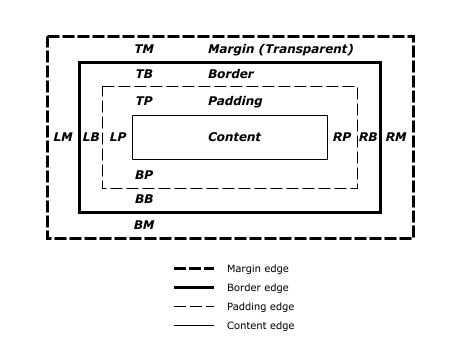
\includegraphics{images/box_model.png}
\par
There are four parts to the box model. From the inside out, they are: content, padding, border, and margin. The content is, as expected, the contents of the element, like text or other elements. The padding is a visible region of the element in which no content can appear. Outside of this is the border which marks the end of the element's visible region. The last component of the box model is the margin, or a region in which other (statically positioned) elements can not exist.
\par
Each of these properties can be set using a shorthand property like \texttt{margin: 20px} or \texttt{border: 2px solid black}. Additionally, by using the \texttt{-left}, \texttt{-top}, \texttt{-bottom}, and \texttt{-right} modifiers, the sizes (and colors and styles, in the case of borders) of the components' constituent parts can be set individually (for instance, \texttt{padding-top:10px; padding-bottom:20px; }).

\subsection{Positioning}

Other than the ubiquitous \texttt{inherit} value, the \texttt{position} CSS property can be either static, relative, absolute, or fixed. \texttt{static} is the default and causes the element to be positioned according to the usual rules. 
\par
For the next three, positioning is accomplished using the \texttt{top}/\texttt{bottom}, \texttt{left}/\texttt{right}, and \texttt{z-index} properties. The first two groups represent the distance of the element's bounding box's top/bottom and left/right edges from those of its positioning reference. The third determines the order in which the element is drawn; an element with a higher \texttt{z-index} is drawn on top one one with a lower \texttt{z-index}.
\par
A \texttt{position} of \texttt{relative} causes any position changes to be relative to the \texttt{static} position of the element.
\par
An absolutely positioned element is positioned relative to the entire document (the whole page). It is essentially popped out of its parent element(s) and pasted somewhere else on screen.
\par
An element that is \texttt{fixed} is positioned relative to the browser's window so that any change in the document's position (i.e. through scrolling or zooming), does not cause the element to move.
\subsection{Other style attributes}
As with the Selectors section, this is also meant to give you an idea of some of the more interesting CSS properties.
\begin{itemize}
\item \texttt{color}: hex, rgb(), or name
  \\ sets the text color
  \\ ex: \texttt{color: \#beefed; /* a light blue */}
\item \texttt{background-color}: \texttt{hex}, \texttt{rgb()}, or \texttt{name}
  \\ sets the background-color of the element's content and padding
  \\ ex: \texttt{background-color: orange;}
\item \texttt{width}: px or \%
  \\ sets the width of the element's content
\item \texttt{height}: px or \%
  \\ sets the height of the element's content
\item \texttt{border-radius}: px or \%
  \\ sets the radius of the element's corners
  \\ use this to make rounded corners
  \\ be careful, this may be copyrighted
\item \texttt{font-size}: em
\end{itemize}

\end{document}